\documentclass[twoside]{book}

% Packages required by doxygen
\usepackage{fixltx2e}
\usepackage{calc}
\usepackage{doxygen}
\usepackage[export]{adjustbox} % also loads graphicx
\usepackage{graphicx}
\usepackage[utf8]{inputenc}
\usepackage{makeidx}
\usepackage{multicol}
\usepackage{multirow}
\PassOptionsToPackage{warn}{textcomp}
\usepackage{textcomp}
\usepackage[nointegrals]{wasysym}
\usepackage[table]{xcolor}

% Font selection
\usepackage[T1]{fontenc}
\usepackage[scaled=.90]{helvet}
\usepackage{courier}
\usepackage{amssymb}
\usepackage{sectsty}
\renewcommand{\familydefault}{\sfdefault}
\allsectionsfont{%
  \fontseries{bc}\selectfont%
  \color{darkgray}%
}
\renewcommand{\DoxyLabelFont}{%
  \fontseries{bc}\selectfont%
  \color{darkgray}%
}
\newcommand{\+}{\discretionary{\mbox{\scriptsize$\hookleftarrow$}}{}{}}

% Page & text layout
\usepackage{geometry}
\geometry{%
  a4paper,%
  top=2.5cm,%
  bottom=2.5cm,%
  left=2.5cm,%
  right=2.5cm%
}
\tolerance=750
\hfuzz=15pt
\hbadness=750
\setlength{\emergencystretch}{15pt}
\setlength{\parindent}{0cm}
\setlength{\parskip}{3ex plus 2ex minus 2ex}
\makeatletter
\renewcommand{\paragraph}{%
  \@startsection{paragraph}{4}{0ex}{-1.0ex}{1.0ex}{%
    \normalfont\normalsize\bfseries\SS@parafont%
  }%
}
\renewcommand{\subparagraph}{%
  \@startsection{subparagraph}{5}{0ex}{-1.0ex}{1.0ex}{%
    \normalfont\normalsize\bfseries\SS@subparafont%
  }%
}
\makeatother

% Headers & footers
\usepackage{fancyhdr}
\pagestyle{fancyplain}
\fancyhead[LE]{\fancyplain{}{\bfseries\thepage}}
\fancyhead[CE]{\fancyplain{}{}}
\fancyhead[RE]{\fancyplain{}{\bfseries\leftmark}}
\fancyhead[LO]{\fancyplain{}{\bfseries\rightmark}}
\fancyhead[CO]{\fancyplain{}{}}
\fancyhead[RO]{\fancyplain{}{\bfseries\thepage}}
\fancyfoot[LE]{\fancyplain{}{}}
\fancyfoot[CE]{\fancyplain{}{}}
\fancyfoot[RE]{\fancyplain{}{\bfseries\scriptsize Generated by Doxygen }}
\fancyfoot[LO]{\fancyplain{}{\bfseries\scriptsize Generated by Doxygen }}
\fancyfoot[CO]{\fancyplain{}{}}
\fancyfoot[RO]{\fancyplain{}{}}
\renewcommand{\footrulewidth}{0.4pt}
\renewcommand{\chaptermark}[1]{%
  \markboth{#1}{}%
}
\renewcommand{\sectionmark}[1]{%
  \markright{\thesection\ #1}%
}

% Indices & bibliography
\usepackage{natbib}
\usepackage[titles]{tocloft}
\setcounter{tocdepth}{3}
\setcounter{secnumdepth}{5}
\makeindex

% Hyperlinks (required, but should be loaded last)
\usepackage{ifpdf}
\ifpdf
  \usepackage[pdftex,pagebackref=true]{hyperref}
\else
  \usepackage[ps2pdf,pagebackref=true]{hyperref}
\fi
\hypersetup{%
  colorlinks=true,%
  linkcolor=blue,%
  citecolor=blue,%
  unicode%
}

% Custom commands
\newcommand{\clearemptydoublepage}{%
  \newpage{\pagestyle{empty}\cleardoublepage}%
}

\usepackage{caption}
\captionsetup{labelsep=space,justification=centering,font={bf},singlelinecheck=off,skip=4pt,position=top}

%===== C O N T E N T S =====

\begin{document}

% Titlepage & ToC
\hypersetup{pageanchor=false,
             bookmarksnumbered=true,
             pdfencoding=unicode
            }
\pagenumbering{roman}
\begin{titlepage}
\vspace*{7cm}
\begin{center}%
{\Large My Project }\\
\vspace*{1cm}
{\large Generated by Doxygen 1.8.11}\\
\end{center}
\end{titlepage}
\clearemptydoublepage
\tableofcontents
\clearemptydoublepage
\pagenumbering{arabic}
\hypersetup{pageanchor=true}

%--- Begin generated contents ---
\chapter{File Index}
\section{File List}
Here is a list of all files with brief descriptions\+:\begin{DoxyCompactList}
\item\contentsline{section}{\hyperlink{Lab1_8c}{Lab1.\+c} }{\pageref{Lab1_8c}}{}
\end{DoxyCompactList}

\chapter{File Documentation}
\hypertarget{Stenciltst_8c}{}\section{Stenciltst.\+c File Reference}
\label{Stenciltst_8c}\index{Stenciltst.\+c@{Stenciltst.\+c}}
{\ttfamily \#include $<$stdio.\+h$>$}\\*
{\ttfamily \#include $<$stdlib.\+h$>$}\\*
{\ttfamily \#include $<$string.\+h$>$}\\*
Include dependency graph for Stenciltst.\+c\+:
\nopagebreak
\begin{figure}[H]
\begin{center}
\leavevmode
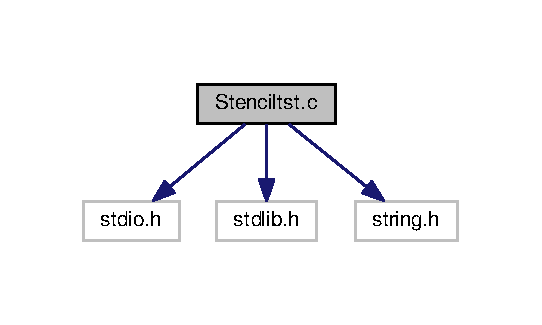
\includegraphics[width=260pt]{Stenciltst_8c__incl}
\end{center}
\end{figure}
\subsection*{Functions}
\begin{DoxyCompactItemize}
\item 
static void \hyperlink{Stenciltst_8c_a97a5364016a0d5bfc018a01db34ca034}{Key} (unsigned char key, int x, int y)
\item 
static void \hyperlink{Stenciltst_8c_a58d1825f5ad50df4f4e09d331d0f1a43}{Draw} (void)
\item 
static void \hyperlink{Stenciltst_8c_ae4d2f7b1f042e0029169e5c2b6c8f02a}{Args} (int argc, char $\ast$$\ast$argv)
\item 
int \hyperlink{Stenciltst_8c_a3c04138a5bfe5d72780bb7e82a18e627}{main} (int argc, char $\ast$$\ast$argv)
\end{DoxyCompactItemize}
\subsection*{Variables}
\begin{DoxyCompactItemize}
\item 
int \hyperlink{Stenciltst_8c_aa1d095ba4bc71c21a758300959a09d2c}{double\+Buffer}
\end{DoxyCompactItemize}


\subsection{Function Documentation}
\index{Stenciltst.\+c@{Stenciltst.\+c}!Args@{Args}}
\index{Args@{Args}!Stenciltst.\+c@{Stenciltst.\+c}}
\subsubsection[{\texorpdfstring{Args(int argc, char $\ast$$\ast$argv)}{Args(int argc, char **argv)}}]{\setlength{\rightskip}{0pt plus 5cm}static void Args (
\begin{DoxyParamCaption}
\item[{int}]{argc, }
\item[{char $\ast$$\ast$}]{argv}
\end{DoxyParamCaption}
)\hspace{0.3cm}{\ttfamily [static]}}\hypertarget{Stenciltst_8c_ae4d2f7b1f042e0029169e5c2b6c8f02a}{}\label{Stenciltst_8c_ae4d2f7b1f042e0029169e5c2b6c8f02a}

\begin{DoxyCode}
110 \{
111   \textcolor{comment}{//GLint }
112 \textcolor{keywordtype}{int} i;
113 
114   \hyperlink{Stenciltst_8c_aa1d095ba4bc71c21a758300959a09d2c}{doubleBuffer} = 1; \textcolor{comment}{//GL\_TRUE;}
115   \textcolor{keywordflow}{for} (i = 1; i < argc; i++) \{
116     \textcolor{keywordflow}{if} (strcmp(argv[i], \textcolor{stringliteral}{"-sb"}) == 0) \{
117       \hyperlink{Stenciltst_8c_aa1d095ba4bc71c21a758300959a09d2c}{doubleBuffer} = 0; \textcolor{comment}{//GL\_FALSE;}
118     \} \textcolor{keywordflow}{else} \textcolor{keywordflow}{if} (strcmp(argv[i], \textcolor{stringliteral}{"-db"}) == 0) \{
119       \hyperlink{Stenciltst_8c_aa1d095ba4bc71c21a758300959a09d2c}{doubleBuffer} = 1; \textcolor{comment}{//GL\_TRUE;}
120     \}
121   \}
122 \}
\end{DoxyCode}
\index{Stenciltst.\+c@{Stenciltst.\+c}!Draw@{Draw}}
\index{Draw@{Draw}!Stenciltst.\+c@{Stenciltst.\+c}}
\subsubsection[{\texorpdfstring{Draw(void)}{Draw(void)}}]{\setlength{\rightskip}{0pt plus 5cm}static void Draw (
\begin{DoxyParamCaption}
\item[{void}]{}
\end{DoxyParamCaption}
)\hspace{0.3cm}{\ttfamily [static]}}\hypertarget{Stenciltst_8c_a58d1825f5ad50df4f4e09d331d0f1a43}{}\label{Stenciltst_8c_a58d1825f5ad50df4f4e09d331d0f1a43}

\begin{DoxyCode}
61 \{
62   \textcolor{comment}{//glClear(//GL\_COLOR\_BUFFER\_BIT | //GL\_STENCIL\_BUFFER\_BIT);}
63 
64   \textcolor{comment}{//glStencilFunc(//GL\_ALWAYS, 1, 1);}
65   \textcolor{comment}{//glStencilOp(//GL\_KEEP, //GL\_KEEP, //GL\_REPLACE);}
66 
67   \textcolor{comment}{/* red trian//gle */}
68   \textcolor{comment}{//glColor3ub(200, 0, 0);}
69   \textcolor{comment}{//glBegin(//GL\_POLYGON);}
70   \textcolor{comment}{//glVertex3i(-4, -4, 0);}
71   \textcolor{comment}{//glVertex3i(4, -4, 0);}
72   \textcolor{comment}{//glVertex3i(0, 4, 0);}
73   \textcolor{comment}{//glEnd();}
74 
75   \textcolor{comment}{//glStencilFunc(//GL\_EQUAL, 1, 1);}
76   \textcolor{comment}{//glStencilOp(//GL\_INCR, //GL\_KEEP, //GL\_DECR);}
77 
78   \textcolor{comment}{/* green square */}
79   \textcolor{comment}{//glColor3ub(0, 200, 0);}
80   \textcolor{comment}{//glBegin(//GL\_POLYGON);}
81   \textcolor{comment}{//glVertex3i(3, 3, 0);}
82   \textcolor{comment}{//glVertex3i(-3, 3, 0);}
83   \textcolor{comment}{//glVertex3i(-3, -3, 0);}
84   \textcolor{comment}{//glVertex3i(3, -3, 0);}
85   \textcolor{comment}{//glEnd();}
86 
87   \textcolor{comment}{//glStencilFunc(//GL\_EQUAL, 1, 1);}
88   \textcolor{comment}{//glStencilOp(//GL\_KEEP, //GL\_KEEP, //GL\_KEEP);}
89 
90   \textcolor{comment}{/* blue square */}
91   \textcolor{comment}{//glColor3ub(0, 0, 200);}
92   \textcolor{comment}{//glBegin(//GL\_POLYGON);}
93   \textcolor{comment}{//glVertex3i(3, 3, 0);}
94   \textcolor{comment}{//glVertex3i(-3, 3, 0);}
95   \textcolor{comment}{//glVertex3i(-3, -3, 0);}
96   \textcolor{comment}{//glVertex3i(3, -3, 0);}
97   \textcolor{comment}{//glEnd();}
98 
99   \textcolor{keywordflow}{if} (\hyperlink{Stenciltst_8c_aa1d095ba4bc71c21a758300959a09d2c}{doubleBuffer}) \{
100     \textcolor{comment}{//glutSwapBuffers();}
101     \textcolor{keywordtype}{int} i;
102   \} \textcolor{keywordflow}{else} \{
103     \textcolor{keywordtype}{int} j;
104     \textcolor{comment}{//glFlush();}
105   \}
106 \}
\end{DoxyCode}
\index{Stenciltst.\+c@{Stenciltst.\+c}!Key@{Key}}
\index{Key@{Key}!Stenciltst.\+c@{Stenciltst.\+c}}
\subsubsection[{\texorpdfstring{Key(unsigned char key, int x, int y)}{Key(unsigned char key, int x, int y)}}]{\setlength{\rightskip}{0pt plus 5cm}static void Key (
\begin{DoxyParamCaption}
\item[{unsigned char}]{key, }
\item[{int}]{x, }
\item[{int}]{y}
\end{DoxyParamCaption}
)\hspace{0.3cm}{\ttfamily [static]}}\hypertarget{Stenciltst_8c_a97a5364016a0d5bfc018a01db34ca034}{}\label{Stenciltst_8c_a97a5364016a0d5bfc018a01db34ca034}

\begin{DoxyCode}
52 \{
53   \textcolor{keywordflow}{switch} (key) \{
54   \textcolor{keywordflow}{case} 27:
55     exit(0);
56   \}
57 \}
\end{DoxyCode}
\index{Stenciltst.\+c@{Stenciltst.\+c}!main@{main}}
\index{main@{main}!Stenciltst.\+c@{Stenciltst.\+c}}
\subsubsection[{\texorpdfstring{main(int argc, char $\ast$$\ast$argv)}{main(int argc, char **argv)}}]{\setlength{\rightskip}{0pt plus 5cm}int main (
\begin{DoxyParamCaption}
\item[{int}]{argc, }
\item[{char $\ast$$\ast$}]{argv}
\end{DoxyParamCaption}
)}\hypertarget{Stenciltst_8c_a3c04138a5bfe5d72780bb7e82a18e627}{}\label{Stenciltst_8c_a3c04138a5bfe5d72780bb7e82a18e627}

\begin{DoxyCode}
126 \{
127   \textcolor{comment}{//GLenum type;}
128 
129   \textcolor{comment}{//glutInit(&argc, argv);}
130   \hyperlink{Stenciltst_8c_ae4d2f7b1f042e0029169e5c2b6c8f02a}{Args}(argc, argv);
131 
132   \textcolor{comment}{//type = //GLUT\_RGB | //GLUT\_STENCIL;}
133     \textcolor{comment}{//type |= (doubleBuffer) ? //GLUT\_DOUBLE : //GLUT\_SIN//GLE;}
134   \textcolor{comment}{//glutInitDisplayMode(type);}
135   \textcolor{comment}{//glutCreateWindow("Stencil Test");}
136 
137   \textcolor{comment}{//glClearColor(0.0, 0.0, 0.0, 0.0);}
138   \textcolor{comment}{//glClearStencil(0);}
139   \textcolor{comment}{//glStencilMask(1);}
140   \textcolor{comment}{//glEnable(//GL\_STENCIL\_TEST);}
141 
142   \textcolor{comment}{//glMatrixMode(//GL\_PROJECTION);}
143   \textcolor{comment}{//glLoadIdentity();}
144   \textcolor{comment}{//glOrtho(-5.0, 5.0, -5.0, 5.0, -5.0, 5.0);}
145   \textcolor{comment}{//glMatrixMode(//GL\_MODELVIEW);}
146 
147   \textcolor{comment}{//glutKeyboardFunc(Key);}
148   \textcolor{comment}{//glutDisplayFunc(Draw);}
149   \textcolor{comment}{//glutMainLoop();}
150   \textcolor{keywordflow}{return} 0;             \textcolor{comment}{/* ANSI C requires main to return int. */}
151 \}
\end{DoxyCode}


Here is the call graph for this function\+:
\nopagebreak
\begin{figure}[H]
\begin{center}
\leavevmode
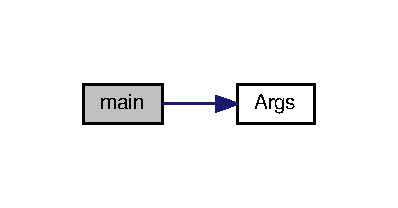
\includegraphics[width=191pt]{Stenciltst_8c_a3c04138a5bfe5d72780bb7e82a18e627_cgraph}
\end{center}
\end{figure}




\subsection{Variable Documentation}
\index{Stenciltst.\+c@{Stenciltst.\+c}!double\+Buffer@{double\+Buffer}}
\index{double\+Buffer@{double\+Buffer}!Stenciltst.\+c@{Stenciltst.\+c}}
\subsubsection[{\texorpdfstring{double\+Buffer}{doubleBuffer}}]{\setlength{\rightskip}{0pt plus 5cm}int double\+Buffer}\hypertarget{Stenciltst_8c_aa1d095ba4bc71c21a758300959a09d2c}{}\label{Stenciltst_8c_aa1d095ba4bc71c21a758300959a09d2c}
(c) Copyright 1993, Silicon Graphics, Inc. A\+LL R\+I\+G\+H\+TS R\+E\+S\+E\+R\+V\+ED Permission to use, copy, modify, and distribute this software for any purpose and without fee is hereby granted, provided that the above copyright notice appear in all copies and that both the copyright notice and this permission notice appear in supporting documentation, and that the name of Silicon Graphics, Inc. not be used in advertising or publicity pertaining to distribution of the software without specific, written prior permission.

T\+HE M\+A\+T\+E\+R\+I\+AL E\+M\+B\+O\+D\+I\+ED ON T\+H\+IS S\+O\+F\+T\+W\+A\+RE IS P\+R\+O\+V\+I\+D\+ED TO Y\+OU \char`\"{}\+A\+S-\/\+I\+S\char`\"{} A\+ND W\+I\+T\+H\+O\+UT W\+A\+R\+R\+A\+N\+TY OF A\+NY K\+I\+ND, E\+X\+P\+R\+E\+SS, I\+M\+P\+L\+I\+ED OR O\+T\+H\+E\+R\+W\+I\+SE, I\+N\+C\+L\+U\+D\+I\+NG W\+I\+T\+H\+O\+UT L\+I\+M\+I\+T\+A\+T\+I\+ON, A\+NY W\+A\+R\+R\+A\+N\+TY OF M\+E\+R\+C\+H\+A\+N\+T\+A\+B\+I\+L\+I\+TY OR F\+I\+T\+N\+E\+SS F\+OR A P\+A\+R\+T\+I\+C\+U\+L\+AR P\+U\+R\+P\+O\+SE. IN NO E\+V\+E\+NT S\+H\+A\+LL S\+I\+L\+I\+C\+ON G\+R\+A\+P\+H\+I\+CS, I\+NC. BE L\+I\+A\+B\+LE TO Y\+OU OR A\+N\+Y\+O\+NE E\+L\+SE F\+OR A\+NY D\+I\+R\+E\+CT, S\+P\+E\+C\+I\+AL, I\+N\+C\+I\+D\+E\+N\+T\+AL, I\+N\+D\+I\+R\+E\+CT OR C\+O\+N\+S\+E\+Q\+U\+E\+N\+T\+I\+AL D\+A\+M\+A\+G\+ES OF A\+NY K\+I\+ND, OR A\+NY D\+A\+M\+A\+G\+ES W\+H\+A\+T\+S\+O\+E\+V\+ER, I\+N\+C\+L\+U\+D\+I\+NG W\+I\+T\+H\+O\+UT L\+I\+M\+I\+T\+A\+T\+I\+ON, L\+O\+SS OF P\+R\+O\+F\+IT, L\+O\+SS OF U\+SE, S\+A\+V\+I\+N\+GS OR R\+E\+V\+E\+N\+UE, OR T\+HE C\+L\+A\+I\+MS OF T\+H\+I\+RD P\+A\+R\+T\+I\+ES, W\+H\+E\+T\+H\+ER OR N\+OT S\+I\+L\+I\+C\+ON G\+R\+A\+P\+H\+I\+CS, I\+NC. H\+AS B\+E\+EN A\+D\+V\+I\+S\+ED OF T\+HE P\+O\+S\+S\+I\+B\+I\+L\+I\+TY OF S\+U\+CH L\+O\+SS, H\+O\+W\+E\+V\+ER C\+A\+U\+S\+ED A\+ND ON A\+NY T\+H\+E\+O\+RY OF L\+I\+A\+B\+I\+L\+I\+TY, A\+R\+I\+S\+I\+NG O\+UT OF OR IN C\+O\+N\+N\+E\+C\+T\+I\+ON W\+I\+TH T\+HE P\+O\+S\+S\+E\+S\+S\+I\+ON, U\+SE OR P\+E\+R\+F\+O\+R\+M\+A\+N\+CE OF T\+H\+IS S\+O\+F\+T\+W\+A\+RE.

US Government Users Restricted Rights Use, duplication, or disclosure by the Government is subject to restrictions set forth in F\+AR 52.\+227.\+19(c)(2) or subparagraph (c)(1)(ii) of the Rights in Technical Data and Computer Software clause at D\+F\+A\+RS 252.\+227-\/7013 and/or in similar or successor clauses in the F\+AR or the D\+OD or N\+A\+SA F\+AR Supplement. Unpublished-- rights reserved under the copyright laws of the United States. Contractor/manufacturer is Silicon Graphics, Inc., 2011 N. Shoreline Blvd., Mountain View, CA 94039-\/7311.

Open\+G\+L(\+T\+M) is a trademark of Silicon Graphics, Inc. 
%--- End generated contents ---

% Index
\backmatter
\newpage
\phantomsection
\clearemptydoublepage
\addcontentsline{toc}{chapter}{Index}
\printindex

\end{document}
